\chapter{Introduction}
\label{ch:intro}

\begin{quote}

`A Machine Learning algorithm walks into a bar.

The bartender asks, `What'll you have?'

The algorithm says, `What's everyone else having?'' \citep{haase2017bar} \end{quote}

This joke by Chet Haase, typifies what is an almost universal axiom in machine learning practice and research. 
Real-world data, a.k.a the ground truth, contains all the information needed for our algorithms to learn from. 
These algorithms should learn to mimic and imitate this data in an unquestioning and uncritical fashion, because real-world data, collected, created or labelled by humans, is all they will need to achieve the aims that we determine they should strive for.

This ethos applies to almost all machine learning research and development. In the context of generative machine learning research, imitating data has led to great success. 
Realistic synthesis of images \citep{karras2019style}, text \citep{radford2018improving}, audio \citep{oord2016wavenet} and video \citep{openai2024sora} were all greatly improved through this approach. 
Striving for realism, however, is not necessarily always a primary creative goal, and in many creative and technological contexts, realism is often considered secondary to other outcomes \textbf{(REF)}. 
Non-photographic rendering is widespread in video games and VfX and underpins the success of many of the most famous games and animated feature films. 
In music, the creative (mis)use of electronic and digital musical instruments, originally designed to imitate traditional instruments, has spawned many musical genres. In addition, tools like digital audio workstations have fundamentally changed the way that people produce, perform, and listen to music.
\textbf{Add references here}.

Achieving realism is not the only goal of generative AI research. 
A number of researchers in the field use datasets of paintings or recordings of musical instruments to train their AI systems. 
The art collective Obvious Art famously sold an AI-generated artwork \textit{Edmond de Belamy} at the Christies auction house for \$432,500 \citep{christies2018edmond}.
The project was completed by creating a dataset of traditional Western paintings and training a generative neural network (REF) on this dataset. 
A new \textit{`painting’} was created by cherry-picking an generated output from this generative model and was then digitally printed onto canvas and adorned in a gilded frame, resurrecting an antiquated practice that dates back to the Renaissance that peaked in 18th and 19th century Europe, where aesthetic and cultural value is prescribed to painted works by placing them in ornate, highly decorated frames.

While training generative AI on paintings is not the same goal as achieving photorealism (though they are imitating digitised photographic images of physical works), this type of work still aims to imitate the representations of real-world phenomena. Here, we are imitating the representations of traditional hand-crafted works, often those that have historical and cultural value.

There have been some attempts to make generative AI produce more creative outputs. 
Continuing with the theme of generating paintings, the ‘Creative Adversarial Networks’ (CAN) algorithm was designed to create ‘original artworks’ with ‘new styles’, by training the AI to deviate from the categories of historical art movements, but to still generate images that look like paintings \cite{elgammal2017can}. 
This research was released to much fanfare and was even featured in an episode of HBO’s Silicon Valley sitcom \citep{elhoseiny2019hbo}. 
However, Jerry Salz, the art critic for the New York Times, was less enthusiastic about the originality of the works generated by this algorithm. 
In a video produced for Vice magazine, he describes one of these CAN generated paintings as being “incredibly dull, generic, boring [...] If the ultimate test is could this have been made by a human, the answer is yes, it has been a thousandth to the thousandth time [...] What I feel is bored when I look at it, what I feel is a lack of originality in the idea that generated it” \citep{saltz2018aiart}. 

\section{The Backlash Against AI Art}

``NO TO AI GENERATED IMAGES", was the caption on a widely shared meme (Figure \ref{fig:c1:no-ai-art}) that was posted to artstation, DeviantArt and other art platforms where traditional artists would share portfolios of their work as a protest to the proliferation of AI-generated artworks using text to image models which had been trained on data harvested from these very platforms. 

\begin{figure}[!htb]
    \centering
    \captionsetup{justification=centering}
    \includegraphics[width=1\textwidth]{figures/c1_intro/no-ai-art.png}
    \caption['No-AI memes being shared on the platform ArtStation]{Screenshot from the art platform \textit{ArtStation}, where memes with the caption `no to AI generated images' were shared widely in a large backlash to generative AI from traditional creative communities.}
    \label{fig:c1:no-ai-art}
\end{figure}

The outrage was levelled at recent developments in text-to-image models from startups such as \cite{midjourney2023midjourney} and \cite{stability2023stability}, that had been trained on large swathes of data collected from internet, including web platforms designed for people to share their art, as a means of having an online portfolio to raise their public profile, and in many cases, marketing their work for people to buy or to attract freelance work, or to gain employment as an artist, graphic designer, or illustrator.

While text-to-image models have been around for some time, the developments in 2022 with diffusion-based models such as dalle-2 \citep{openai2022dalle2}, MidJourney v4 \citep{edwards2022midjourney} and stable diffusion \citep{stability2022stable}, and their ability to so successfully imitate the existing styles of individual artists, simply by listing the names of well-known creators on these digital platforms in the input text prompt, sparked outrage in the creative communities from which a lot of the data was sourced. 
A large part of the outrage was the use of the entire body of individual artists' works for training data without consent and without remuneration.
There are also legitimate and substantiated fears, that these generative AI systems will put creatives out of work and lower the barrier to entry for image generation so considerably to make it a trivial pursuit requiring little skill or training to produce commercially viable results.

Much of the content shared in protest against AI-art was quoted with statements such as “AI is theft” \citep{whiddington2022backlash}, with trending hashtags like \#SupportHumanArtists \citep{zakuga2022theft}. 
Several ongoing lawsuits have emerged against companies like MidJourney and Stability.AI, from artists themselves \citep{brittain2023artists} and from companies like Getty Images and shutterstock that provide stock photographs and artworks \citep{vincent2023getty}. 
Many artists have now removed their work portfolios from publicly available sites, and artstation and DeviantArt now have metadata tags for ‘NoAI’ \citep{artstation2022noai}, meaning permission is withheld for those works to be used in creating datasets for training AI systems, which users on DeviantArt platforms are opted into by default \citep{deviantart2022optout}. 
This trend of opting out automated webscraping for AI training has been expanded to any website listed on the world wide web, with `ai.txt' files \citep{aitxt2024spawning}. 

Speaking as a researcher and practitioner in the direct field, it is my view the concerns and grievances of these artists are completely legitimate. 
I have been an active member of the CreativeAI community since its inception, and it is disheartening to see 'big tech' startups entering this space and acting with such contempt for the communities of artists from which much of their value and power is sourced. 
The work in this thesis is positioned in opposition and as an alternative to the practices of these large tech organisations. 
The goal of this thesis has been to find new ways of \textit{making} with AI, and find ways of creatively (mis)using these technologies in order to understand them better from the perspective of those in the arts \citep{salvaggio2023aarg}.
Throughout the development of this PhD research, I have sought to explore how we can create using generative AI without imitating data, and in addition, how we can use generative AI to create new styles and sounds without rehashing what humans have already created, and further, how we can learn more about how generative AI works by trying to interfere with its intended operation (\S \ref{ch:net_bend}; \S \ref{c8:sec:explaining}).

\section{Intellectual Property and AI Art}

My first encounters with the issues of copyright, ownership and authorship of work with generative AI predate these developments. 
In 2015-16, I was working towards a research Master's thesis in Creative Computing at Goldsmiths, just as generative AI research was beginning to demonstrate significant improvement in realism. 
In one of the experiments outlined in the thesis, I used all the frames from the film Blade Runner as the training data for an autoencoder model, which after training I used to make a reconstruction of the film through the learned model \citep{broad2016autoencoding} (Figure \ref{fig:c1:blade-runner}).
The film \textit{Blade Runner -- Autoencoded} garnered a large international interest and I was very lucky to have had the work exhibited around the world in major museums and galleries \citep{broad2017autoencoding} (Figure \ref{fig:c1:blade-runner-whitney}).

\begin{figure}[!htb]
    \centering
    \captionsetup{justification=centering}
    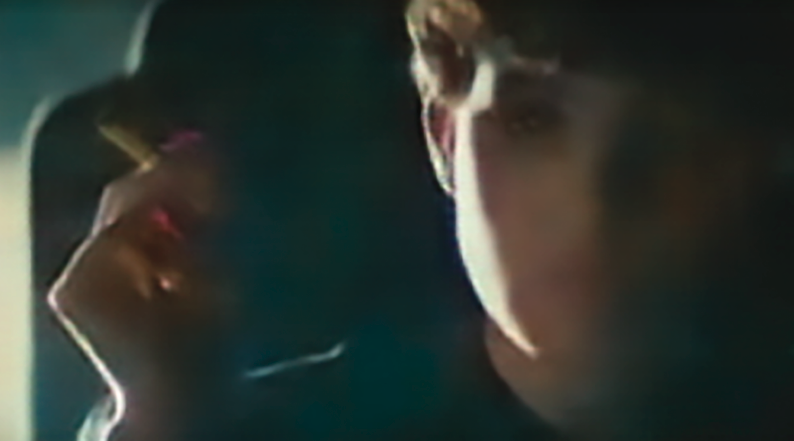
\includegraphics[width=1\textwidth]{figures/c1_intro/blade_runner_still.png}
    \caption{Still from \textit{Blade Runner --- Autoencoded}.}
    \label{fig:c1:blade-runner}
\end{figure}

\begin{figure}[!htb]
    \centering
    \captionsetup{justification=centering}
    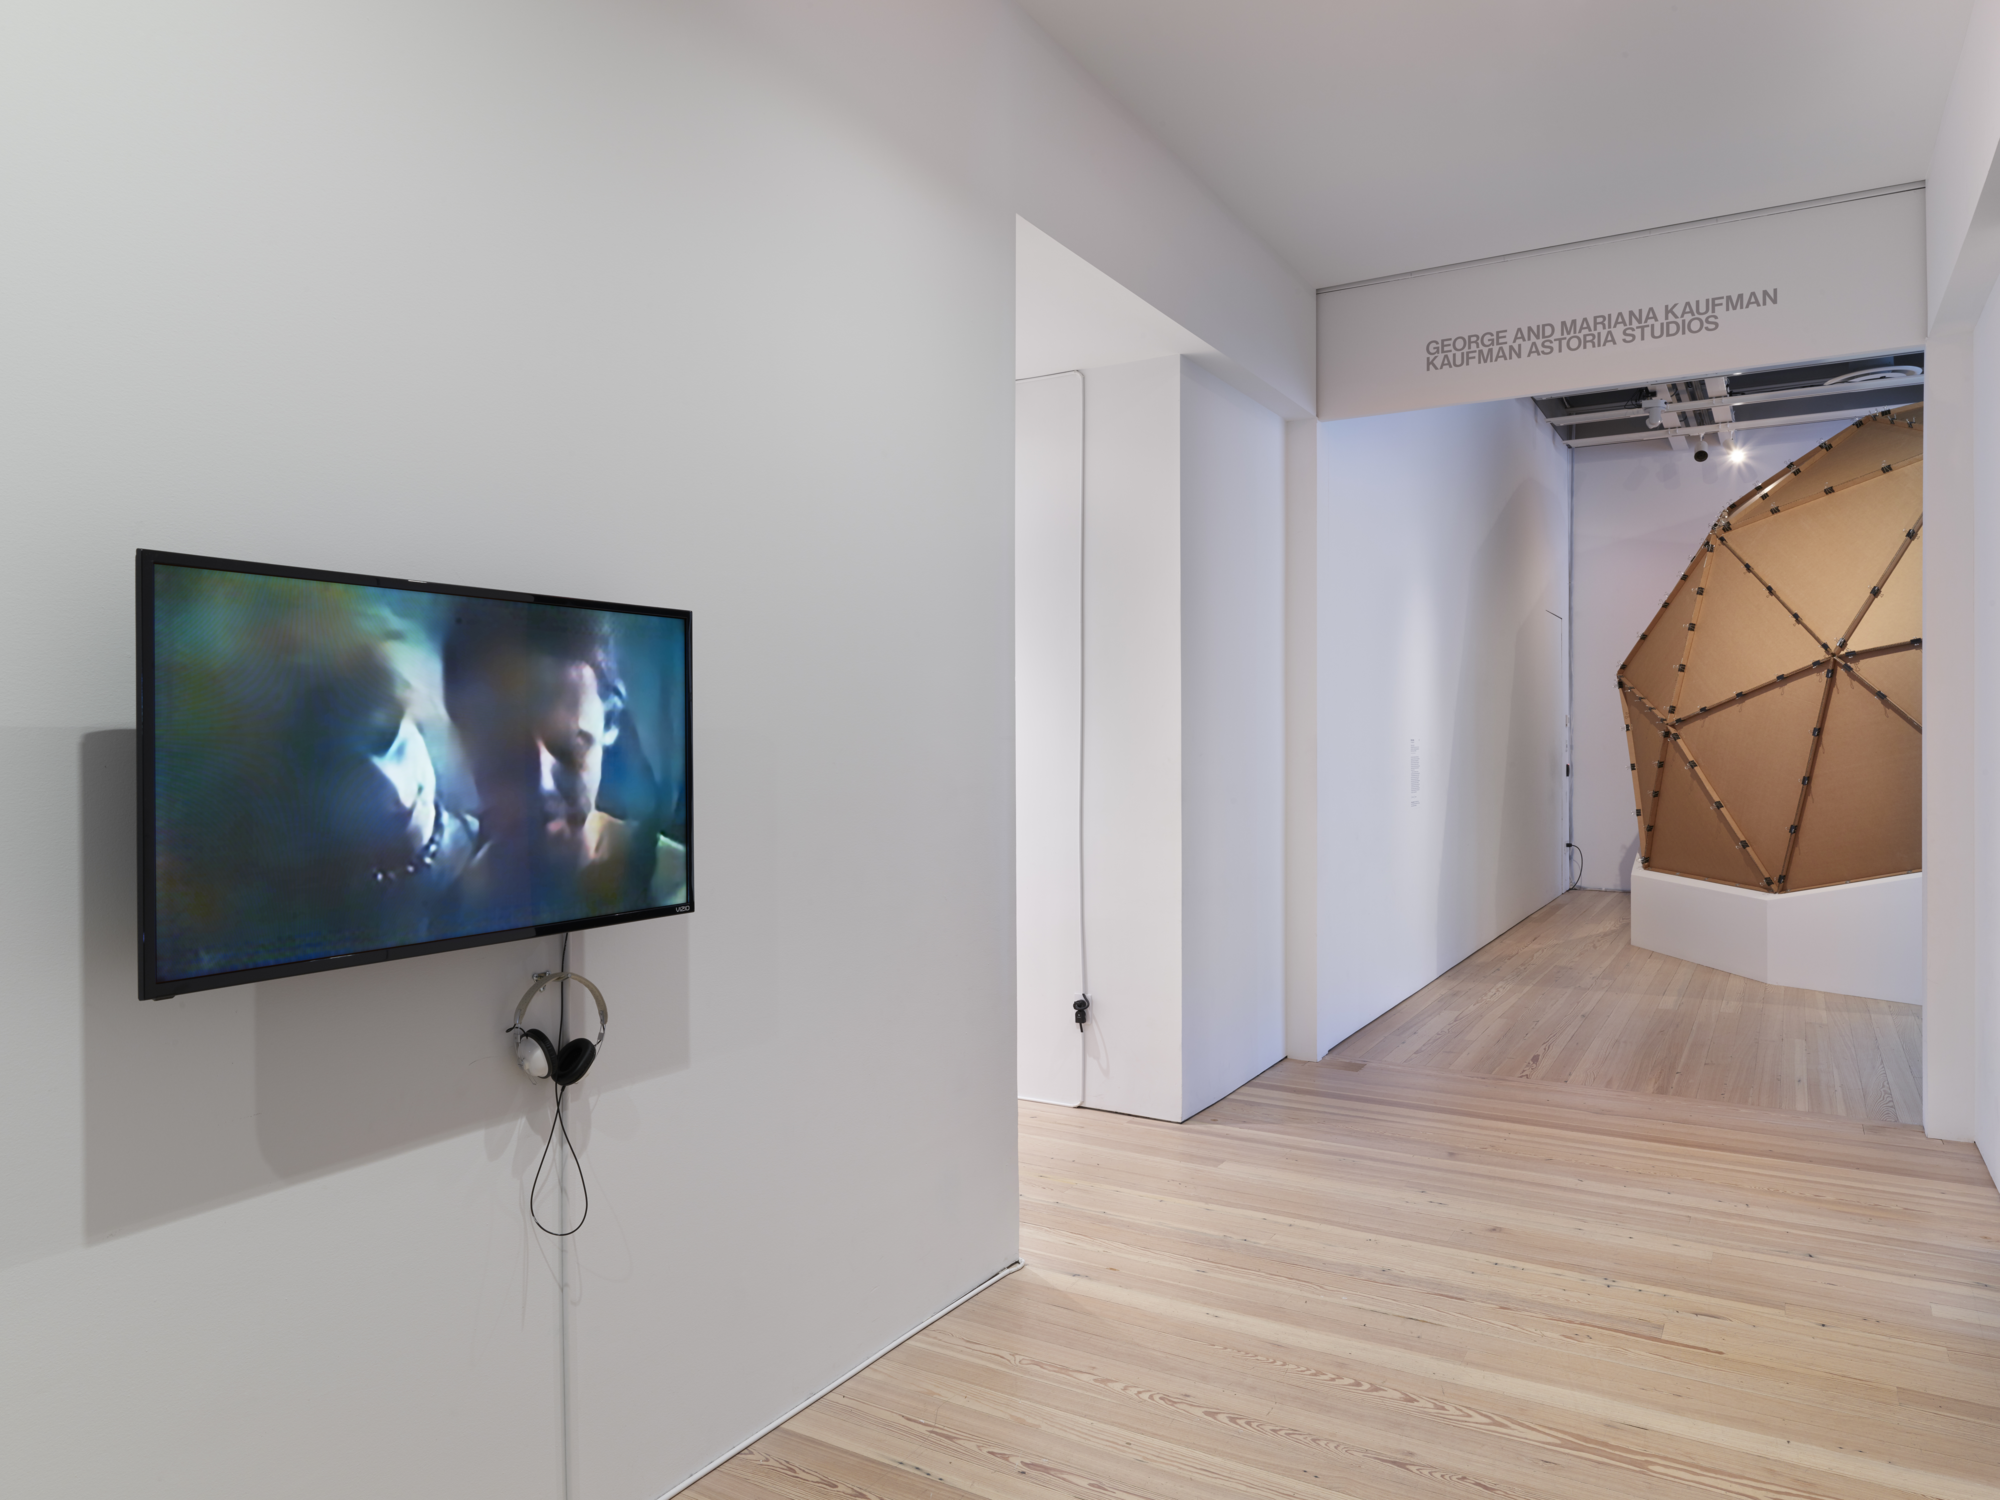
\includegraphics[width=1\textwidth]{figures/c1_intro/whitney-installation-shot.png}
    \caption[Installation shot of of \textit{Blade Runner --- Autoencoded}]{Installation shot of \textit{Blade Runner --- Autoencoded} at the Whitney Museum of American Art (2016). Image courtesy of the Whitney Museum of American Art, photograph by Ron Amstutz (permission to reproduce TBC).}
    \label{fig:c1:blade-runner-whitney}
\end{figure}

The training data, of course, was not intellectual property that I had the permission to use. \footnote{It should also be noted that I was not even the only person to recreate \textit{Blade Runner} with machine learning. Ben Bogart's work \textit{Watching (Blade Runner)} was also created in 2016 \citep{bogart2016watching}, and I only learnt of its existence many months after completing my own recreation of the film.}
Ironically, this project and the resulting (and later rescinded) DMCA copyright takedown notice given to the videos on the web platform Vimeo was what catapulted the work to international recognition after an account of these travails was detailed in the news website Vox \citep{romano2016bladerunner}.

hough I did not face any further legal action from Warner Brothers for  disseminating the work, it was a major cause of personal stress, as I was very often anticipating some form of legal intervention (e.g. a cease and desist notice) from Warner Brothers prior to any exhibition where the work was going to be shown.
An opinion published in the Columbia Journal of Law and the Arts predicted that the work would probably be dealt with as copyright infringement were it tested in an American court \citep{sobel2017artificial}.\footnote{An alternative legal opinion was given by legal scholar Andres Guadamuz, who believed that this would would be protected by fair-use or fair-dealing if it were to be tested in court on the basis of parody or pastiche \citep{guadamuz2024personal}.} 
I produced the work before the widespread emergence of NFTs and before there was a large market for AI-generated artworks. 
The money I made from exhibition fees and selling editions of the video work would have been relatively insignificant for a multinational media company. 
Nonetheless, this experience was instrumental in my research approach. 
Finding ways of using generative AI that does not rely on data and the intellectual property of others was a key aim for the research presented in this thesis

\section{Motivation}

My goal was to find ways of training or configuring generative AI models which did not rely on the creation of datasets to produce creative outcomes. 
From working in industry, I had experienced how labour-intensive and time-consuming creating high-quality datasets could be, and it was clear this was a hugely time-consuming aspect of Generative AI research processes.
The second was to find ways of achieving novel outcomes that did not rely on access to high-end resources, for example those available to large technology companies, including Google DeepMind, NVIDIA, or artists such as Refik Anadol (who reportedly have access to considerable computational resources  \citep{caulfield2022refik}). 
To this end, this research has focussed on exploring methods for training, configuring and customising very high-fidelity models that, when trained conventionally, require supercomputer-level resources. 
As such, this thesis presents a number of useful methods for manipulating, training and controlling these same models in much shorter time periods on consumer-level hardware.


Instead of relying on laboriously or ethically questionable datasets to try and achieve creative outcomes, the work in this thesis details data-free methods that push the possibility space of what can be generated with contemporary neural networks.
The approaches detailed are an attempt to use the intrinsic affordances of these neural networks to create original outputs that would not have been possible using any other technique or technology. 
The work detailed in this thesis is experimental image-making in its truest sense, and I have taken more inspiration from experimental photographers and filmmakers of the 20th Century (such as Harold Edgerton, Hiroshi Sugimoto, and Oskar Fischinger) than from academic researchers.

The driving force that led to each technical breakthrough in this thesis has been technical curiosity. 
When considering a new possible configuration for training an AI or some other kind of intervention, if I couldn’t imagine what the result of that experiment would look like, I would have to build it to find out, regardless of how many weeks or months of work it would take to get there. 
The results presented here are the experiments that produced the most surprising and striking results - sometimes beautiful and sometimes horrifying. 
There were a lot of failed experiments along the way that produced boring, predictable and uninspiring results. 
I’ve spared the reader details of most of these, apart from the few that led to key insights.

\section{Research Methods}

The research breakthroughs presented in this thesis have all come from a technological exploration of what is possible with these new technologies. Much of this research has been conducted in the vein of hacking, in its original meaning from the hacker culture at MIT in the 60s and 70s, where hacking meant “exploring the limits of what is possible, in a spirit of playful cleverness” \citep{stallman2002hacking}. 
This hacking ethos is not an approach that many people were taking in machine learning research when I started this PhD. 
The field was, and still is, very much dominated by orthodoxies and ideology, where theoretical mathematical underpinnings, achieving state-of-the-art performance on some widely used benchmark, and generalisation are most valued by the research communities \citep{birhane2022values}.

\textit{Hacking} was the primary means by which the algorithms in this thesis were discovered, but artistic exploration has also been central to the experimental work described in this thesis. 
When I started this PhD, my plan was to conduct primarily technical research and continue with an artistic practice on the side, maybe using some of the techniques developed in my research. 
Instead, it was an artistic enquiry that led me to the technical breakthroughs in the PhD, not the other way around. 

In his paper \textit{"Art in the sciences of the artificial"}, Stanley argues that in the fields of artificial intelligence research and artificial life, subjective evaluation is a key driving force of progress for many researchers and practitioners in the field. 
There is a tendency in these research fields to discourage the dissemination of these observations in academic writing and in wider public discourse, something that Stanley worries might “cut off some future discoverers from what could have been their inspirations” \citep{stanley2018art}. 
In this thesis, I have sought to share my subjective position at various times in the thesis, and how that informed the direction of the following research experiments (see \S \ref{c8:sec:aesthetic} for a further reflection on this).

Being both guided by, and disseminating this kind of subjectivity is commonplace in research practices in many areas of the humanities, including research methods such as autoethnography \citep{reed1997auto}, or practice-based and practice-led research \citep{candy2006practice}. 

The goal of this research has been at its core, to advance the creative possibilities of these technologies. 
As a practising and internationally recognised visual artist, my subjective understanding of the visual potential and aesthetics of these systems, has been one of the central guiding instruments in this research. 
To give any other account of how this research was conducted would be a failure of academic integrity. 

The work  I have done that is described in this dissertation and the contributions made in this thesis were the outcomes of practice-led research. 
The artistic outcomes are not presented as contributions to be assessed as outcomes of the thesis as such, but the process and practice that went into making them are described in an honest account in this thesis. 
Descriptions of artworks that have been made by myself and others using the techniques that have been described in this thesis are detailed in Chapter \ref{ch:impact}.

\section{Overview and Contributions of the Thesis}

The thesis is entitled \textit{Expanding the Generative Space}. 
The throughline of all of the research presented here has been to find ways of going beyond the imitation of training data as the sole method for training generative neural networks. 
Instead, I have been trying to expand the possibility space that generative AI can produce, and the methods described in this thesis are but a few of the ways that this is possible. 

\subsection{Background}

Chapter \ref{ch:background} provides a thorough review of relevant background literature and related research conducted prior to the work presented in this thesis.
This review encapsulated both the technical aspects of machine learning relevant to this thesis, and also its application in creative contexts, whilst also drawing on the broader history of artificial intelligence methods such as evolutionary algorithms, and their applications for generative processes. 
This chapter also describes notable prior work in relation to attempts to achieve novel outcomes with generative neural networks.

\subsection{Training without Data}

Chapter \ref{ch:unstable_eq} documents the first peer-reviewed and published approach to training generative neural networks without data, one of the three categorical contributions to active divergence methods (\S \ref{survey:nodata}) presented in this thesis.
This work was first published in the paper \textit{`Searching for an (un)stable equilibrium'}: experiments in training generative models without data' at the NeurIPS 2019 Workshop on Machine Learning for Creativity and Design \citep{broad2019searching}.

\subsection{Divergent Fine-Tuning}

Chapter \ref{ch:divergent} documents the first peer-reviewed and published approach to divergent fine-tuning of generative AI models without relying on imitation-based learning.
Divergent fine-tuning is another categorical contribution to active divergence methods (\S \ref{survey:divergent}) presented in this thesis.
This work was first pubished in the paper \textit{`Amplifying the uncanny'} at the 8th Conference on Computation, Communication, Aesthetics \& X (xCoAx) \citep{broad2020amplifying}.


\subsection{Network Bending}

Chapter \ref{ch:net_bend}, presents the network bending framework and is the third categorical contribution to active divergence methods presented in this thesis (\S \ref{survey:bending}).
This work was first published in the paper \textit{`Network Bending: Expressive manipulation of deep generative models'} at the International Conference on Artificial Intelligence in Music, Sound, Art and Design (EvoMUSART)\citep{broad2020network}, and later extended in the paper \textit{`Network Bending: Expressive Manipulation of Generative Models in Multiple Domains'} for the journal Entropy \citep{broad2021network}.
Network bending has been widely reused and adopted by many other artists and researchers (detailed in \S \ref{c7:sec:net-bend-artworks}; \S \ref{c7:sec:net-bend-impact}).

\subsection{Active Divergence Taxonomy}

The final contribution of this thesis is the survey and formal taxonomy. 
The large majority of experimental work in this thesis falls under the umbrella term \textit{active divergence}. 
This was first coined by a PhD colleague and friend, Sebastian Berns and his supervisor Simon Colton [\citeyear{berns2020bridging}]. 
The core experimental work in this thesis pre-dates this definition, and I am indebted to Sebastian for summarising the overarching theme of my research, which felt far more disparate when I was working on it until he was able to summarise it in a two-word definition. 
In collaboration with Sebastian and Simon, I expanded on this definition and the paper ` Active Divergence with Generative Deep Learning - A Survey and Taxonomy' at the International Conference of Computational Creativity in 2021 \citep{broad2021active}.
An updated summary of that survey is presented in Chapter \ref{ch:active_div} and details work completed concurrently by others during the time of this PhD to achieve similar goals.

\subsection{Discussion and Impact}

Chapter \ref{ch:impact} details the impact of the research presented in this thesis and the subsequent work that this thesis went on to inspire. Chapter \ref{ch:discussion} reflects on the work undertaken, how artistic approaches to hacking AI models and training can lead to new forms of understanding, and how AI itself can be used as a material for artistic exploration and expression, a topic that I discussed in the paper \textit{`Using Generative AI as an Artistic Material: A Hacker's Guide'} that I presented at the 2nd international workshop on eXplainable AI for the Arts (XAIxArts) at the ACM Creativity and Cognition Conference \citep{broad2024using}.

\subsection{Conclusion}

Chapter \ref{ch:conclusion} concludes the thesis and reflects further on its contributions.
This chapter also details the limitations of the research presented in this thesis and discusses possible future research directions to take this work further.

\section{Summary}

In the six years that I have been working on this PhD, there has been a huge amount of upheaval in the research field and its impacts on wider society. 
I have seen AI art and generative AI go from a small, quirky community of enthusiasts to a booming industry that has become pitted against the interests and livelihoods of the creative professionals that they are extracting value from.
Hopefully, the approaches to working with AI described in this thesis can help others to find ways of using and working with generative AI which do not rely on the mass stealing and exploitation of creative professionals, but instead fosters new ways for creative people to use generative AI in ways that creatives always will do: to deliberately break, misuse and adapt technologies far beyond the intended purpose to forge new forms of creative expression.
